\documentclass[letterpaper,12pt]{article}
\usepackage[utf8]{inputenc}

\usepackage{rotating}
\usepackage[top=1in, bottom=1in, left=1in, right=1in]{geometry}
\usepackage{graphicx}
\usepackage[numbers,square,sort&compress]{natbib}
\usepackage{setspace}
\usepackage[cdot,mediumqspace,]{SIunits}
\usepackage{hyperref}
\usepackage{mathtools}
\usepackage{url}
\usepackage{authblk}
\usepackage{placeins}
\usepackage{float}

\onehalfspacing
\title{Measuring AU Using Solar Observation}
\author{Anita Bahmanyar \qquad Ayushi Singh \qquad Morten Nyborg Stostad \\Department of Astronomy and Astrophysics, University of Toronto}
\affil{\small {Written by: Anita Bahmanyar}}
\affil{\small {anita.bahmanyar@mail.utoronto.ca}}
\affil{\small {Student Number: 998909098}}
\date{April 4 2014}

\usepackage{graphicx}

\begin{document}

\maketitle

%Abstract
\begin{abstract}
\label{abstract}
In this lab our goal is to measure the distance between Sun and the Earth (AU) in meters using simple geometry. The solar data was taken on March 18, 2014 using the 8 inch refractor telescope located on top of the Burton Tower at University of Toronto. Using Toshiba CCD and spectrometer, we measure the rotational velocity of the sun by computing the Doppler shift between spectra of the limbs of the sun. We used two methods of covariance and Fourier Transform in order to find the wavelength shift between two edges f the sun. Using our calculated rotational velocity of the sun, we estimated AU to be [...] $\pm$ [...] km which is ... \% of the known value.

\section{Introduction}
\label{sec:introduction}
Astronomical distances and scales are large enough that is gets bothersome to use usual distance units such as meters and kilometers. Therefore, astronomers defined a new unit for length measurements called Astronomical Unit(AU), which is defined as the distance between the Sun and the Earth. In this lab we will use simple geometry, circular motion and properties of light to measure this unit. In order to do so, we found the wavelength solution of the Charged Coupled Device(CCD) that related the pixel numbers to wavelengths as explained in section [...], obtained the solar spectra along its diameter and by taking advantage of cross-correlation method as discussed in section [...], we figured out the pixel shift and therefore the Doppler Shift in the solar spectra with respect to the starting point( in order to determine the radial velocity of the Sun. From this, we can compute the radius of the sun by knowing the period of the Sun. Then finally we can compute AU using geometry as will be explained more in section [...]. The goal of this lab is to learn to find the wavelength solution for CCDs, cross-correlate data sets with each other and find the rotational velocity of the sun in order to find its radius and finally to measure AU using simple geometry as described later.


 
\section{Observation and Data Acquisition}
\label{sec:observationanddataacquisition}
\subsection{Neon and Mercury Lamps}
We used HR1 spectrometer which consists of Toshiba 1 $\times$ 3652 CCD. Size of each pixel is 8 $\mu$ $\times$ 200 $\mu$.  The wavelength range of this spectrometer is 523-573 nm. We used Neon and Mercury lamps to find the wavelength solution for this spectrometer. We set the integration times such that the pixels are not saturated. Therefore, we used 200 ms and 400 ms integration time for neon lamp and 10 ms and 50 ms integration times for the mercury lamp. We also took data of dark counts with the same exposure times for each lamp. 
\subsection{Solar Observing}
We went up to 16th floor of Burton Tower to use the 8-inch refractor telescope for our purpose. We mounted another telescope cap in front of the telescope aperture in order to reduce the amount of light coming into telescope from the Sun so that we do not hurt our eyes. Then we mounted the projection screen as it can be seen in Figure 1 so that we get the Sun on the screen. Next step was to line up the shadow of the finder scope until it became circle as in Figure 2 and then focused the the telescope to get a sharp image(We did this by looking at the sharpness of the sun spots). The next thing we need to consider is the temperature of the spectrometer since the spectral resolution and dispersion of the the spectograph or in general, the wavelength solution changes with temperature and for this mean we placed the spectrometer inside a box to keep the temperature approximately as it was in the astronomy lab, where we collected Neon and Mercury data to solve for the wavelength solution. The box consisted of a resistor that heats up the box. Then we connected the fibre coupler to collimate [....] 

% images a and 2 (flat and centroids)
\begin{figure}[ht]
\centering
\begin{minipage}[b]{0.4\linewidth}
  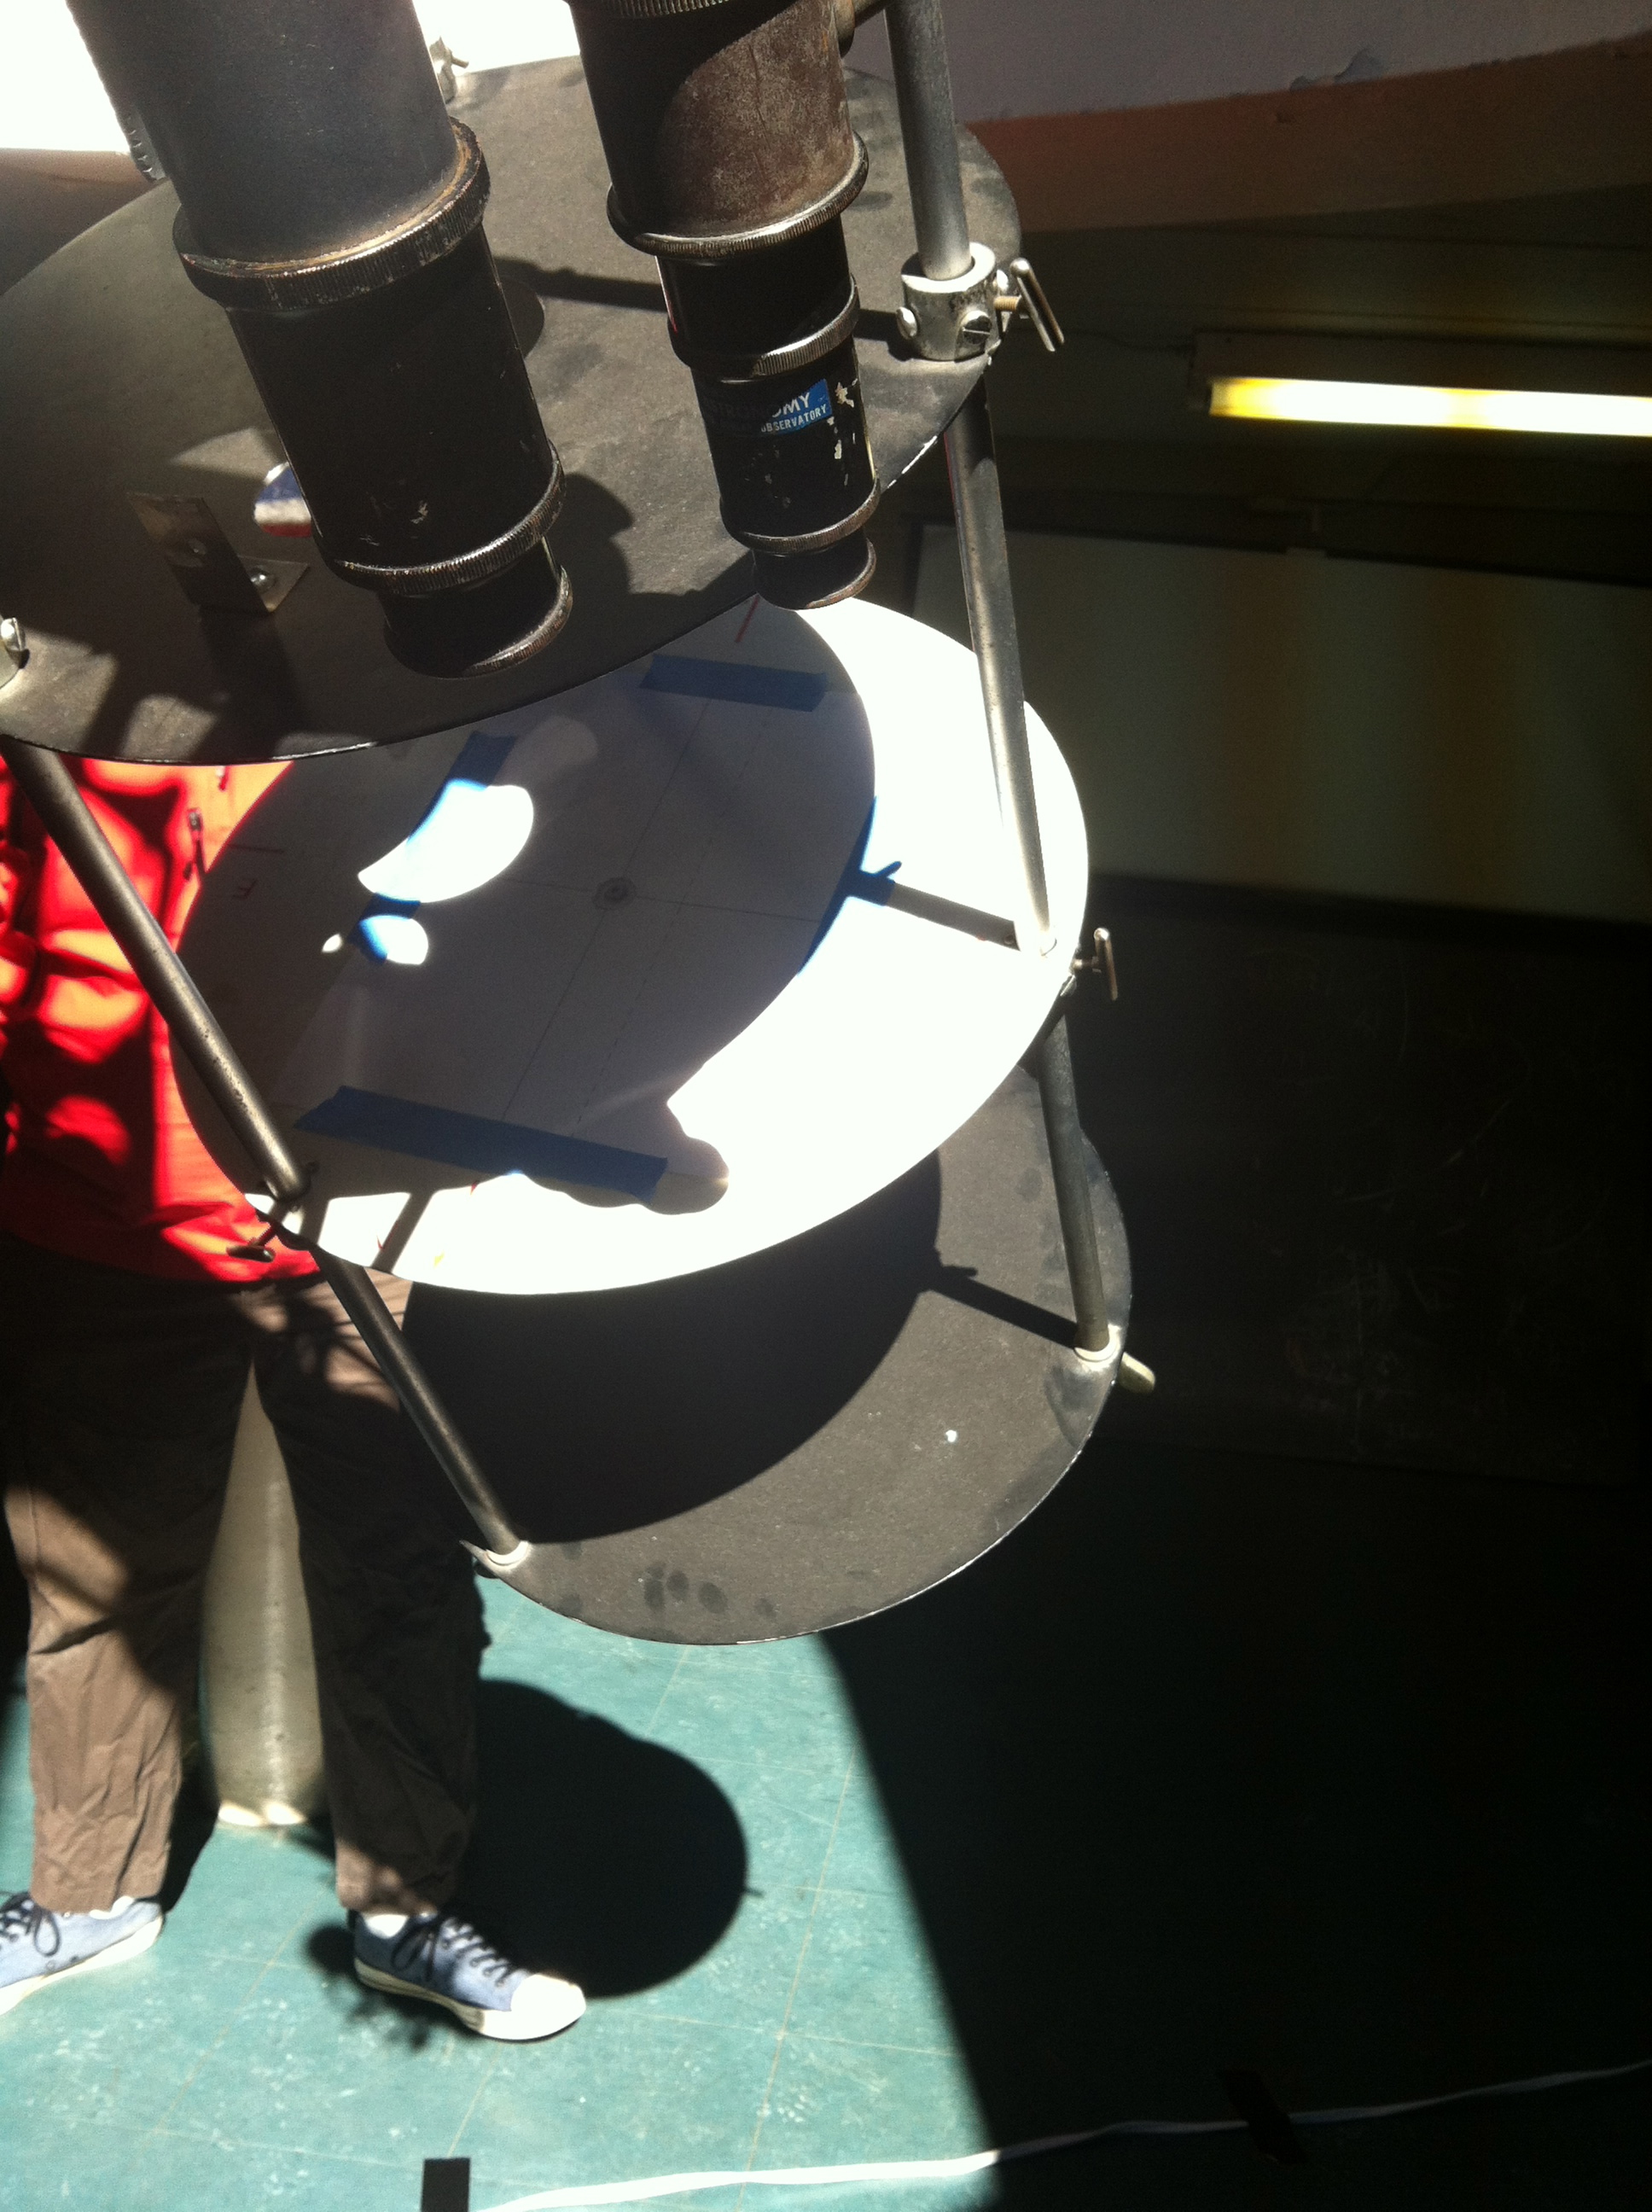
\includegraphics[scale=0.09]{projection.jpg}
  \caption{This figure shows the projection screen mounted on the telescope to get and the image of the Sun on the screen(indirect observing)}
  \label{fig:minipage1}
\end{minipage}
\quad
\begin{minipage}[b]{0.4\linewidth}
  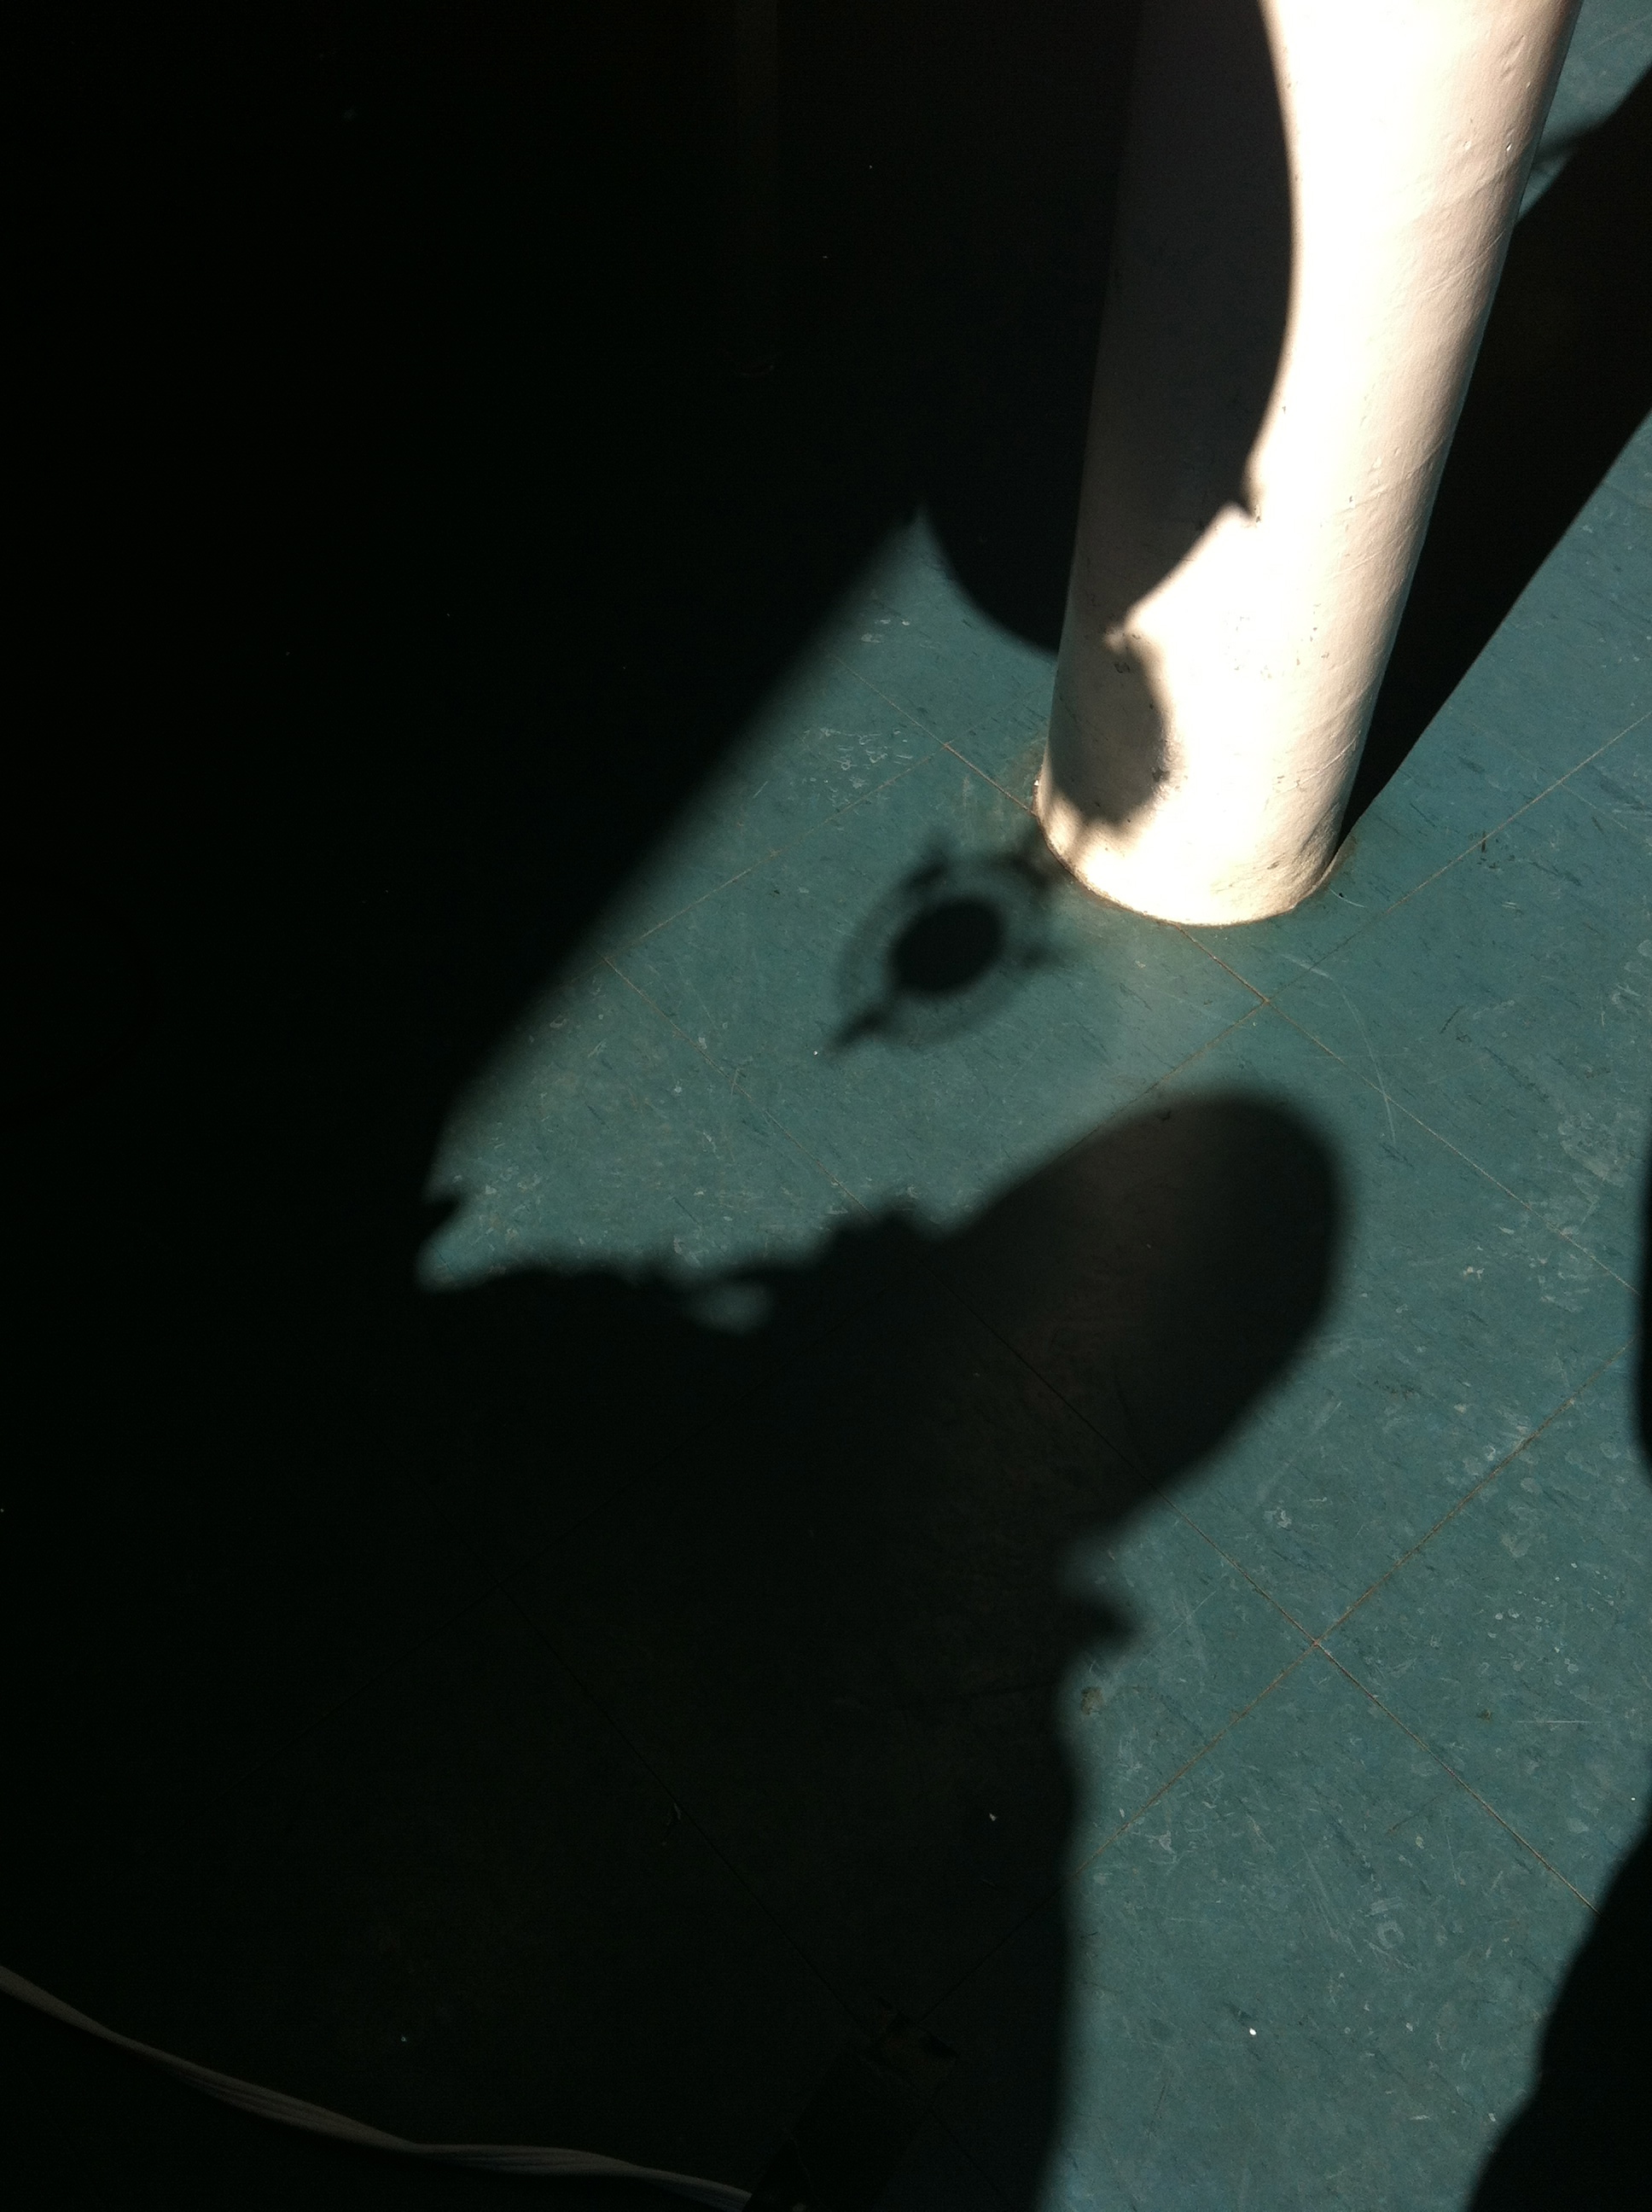
\includegraphics[scale=0.09]{finder-lineup.jpg}
  \caption{This figure shows the shadow of the finder scope as a circle which means it is lined up correctly. We also focused the telescope.}
\label{fig:minipage2}
\end{minipage}
\end{figure}




\section{Analysis}
\label{sec:analysis}
\subsection{Wavelength Solution}
We calibrated the wavelength of the spectrometer since we need to figure out how wavelength is related to the pixel numbers to the wavelength. We used neon and mercury lamps for this purpose. We took 200, 400 and 1000 ms integration times for neon and 10 and 50 ms integration times of data for mercury as well as dark data sets for all of these integration times. We then subtracted dark from the data sets. Figure [....] shows the the intensity vs. pixel number of 10ms mercury and 200ms neon lamp graphs.
We then found the peaks of the graph using centroid method as discussed in Appendix section. Then we compared these peaks with a reference peak wavelength for neon and mercury in the spectrometer wavelength range and plotted the wavelengths vs. pixel numbers in order to find the wavelength solution. We used linear least squares to fit the graph. This was done manually in Python as explained in Appendix, so it means we did not use the built-in package of Python. Fig. [...] shows the wavelength solution, which is $y=0.014 x +524.61$, where $y$ is the wavelength and $x$ is the pixel number. 



\FloatBarrier
\begin{figure}[h!]
\centering
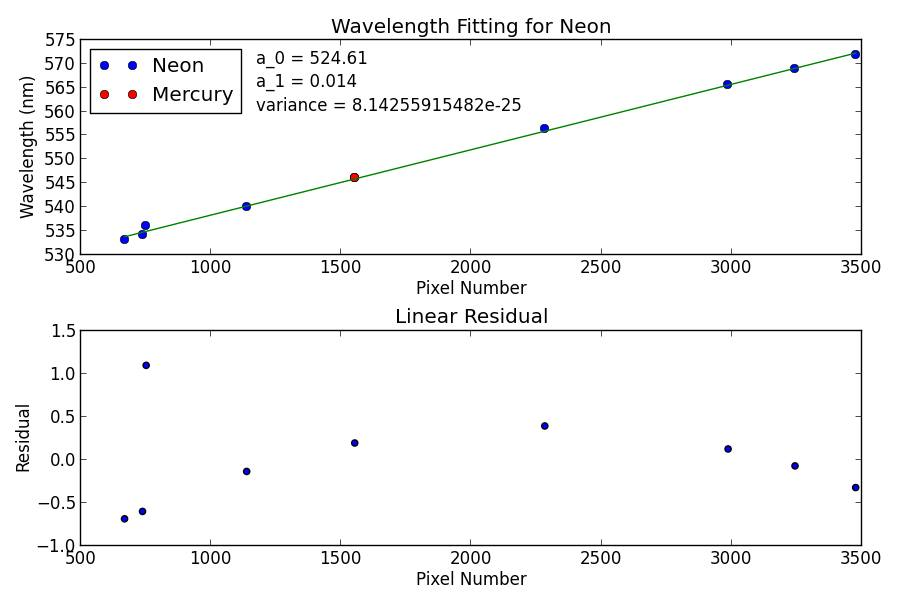
\includegraphics[scale=0.3]{wavelengh_solution.jpg}
\caption{The upper image shows the wavelengths vs. pixel numbers of neon and mercury peaks as compared with their reference spectrum. The wavelength solution is written in the graph. The lower image shows the error in the data and as it is visible it is very small and the variance is also very small that is negligible.}
\end{figure}
\FloatBarrier

Figurea [...] and [...] show the intensity vs. wavelength for neon 200ms and mercury 10ms.

\begin{figure}[ht]
\centering
\begin{minipage}[b]{0.5\linewidth}
  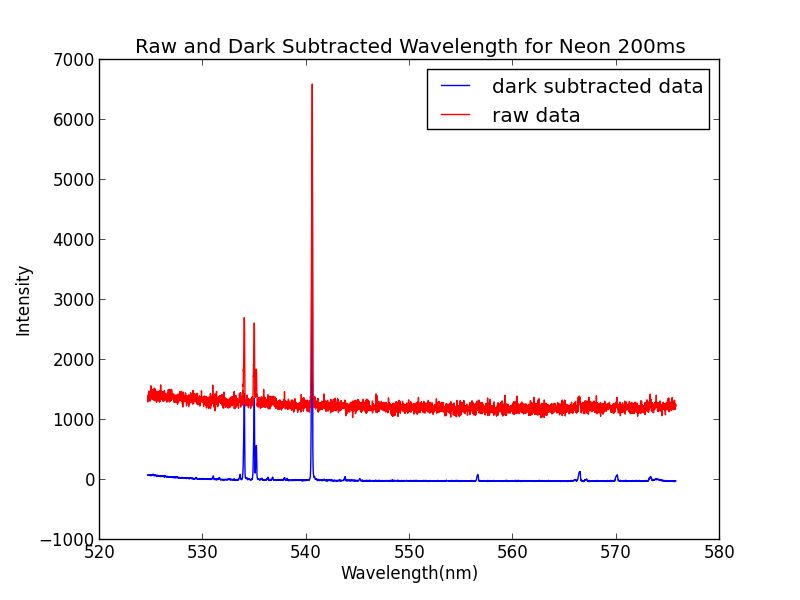
\includegraphics[scale=0.4]{wavelength_neon200ms.png}
  \caption{This figure shows the intensity vs. wavelength of neon 200ms. The raw data is very noisy unlike the mercury raw data.}
  \label{fig:minipage1}
\end{minipage}
\quad
\begin{minipage}[b]{0.4\linewidth}
  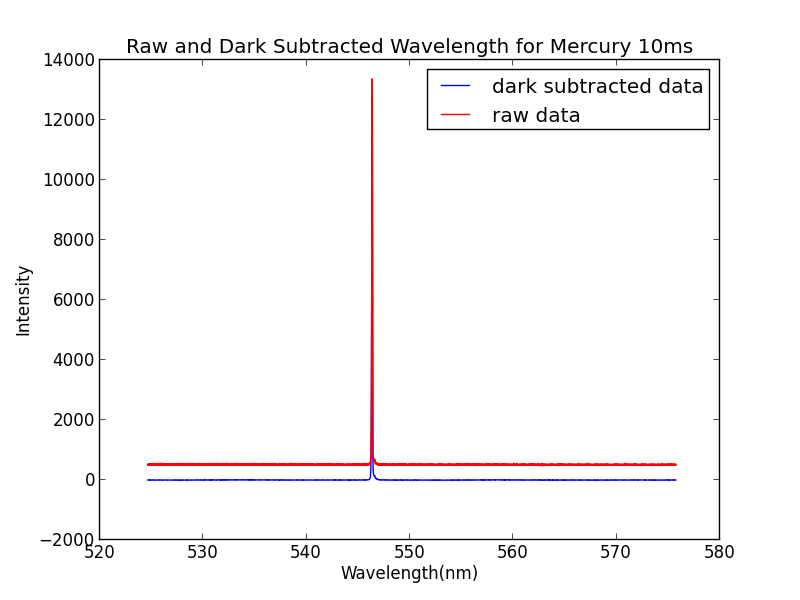
\includegraphics[scale=0.4]{wavelength_merc10ms.png}
  \caption{This figure shows the intensity vs. wavelength of mercury 10ms.}
\label{fig:minipage2}
\end{minipage}
\end{figure}

\subsection{Solar Data}
After finding the wavelength solution of the spectrometer, we should work with solar data. One of the solar data spectrums is plotted vs. wavelength in Fig. [...].



We collected 170ms and 200ms data sets on March 13, 2014 and three sets of data with 125ms integration time on March 18, 2014. We found the mean of each data file and plotted these mean values vs. time. The times where extracted from the file names as it will be discussed in details in Appendix. Then we considered the limb darkening which is given by equation [...]:

\begin{equation}
I=\frac{2}{5}I_{0}(\frac{3}{5}+\sqrt{\frac{(t-t_{0})^2}{\Delta t^2}})
\end{equation}

$I_{0}$ is the intensity of the center value, $\Delta t$ is the difference in the time of the two start and end point data and $t_{0}$ is the time of the central data.


% table showing the t and delta values with their errors
\FloatBarrier
\begin{table}[h!]
\caption{Limb Darkening Parameters} % title of Table
\centering % used for centering table
\begin{tabular}{| c | c | c | c | } % centered columns (4 columns)
\hline %inserts double horizontal lines
  & $I_{0}$& $t_{center} [s]$ &  $\Delta t$ [s]\\ [0.5ex] % inserts table

%heading
\hline % inserts single horizontal line
                   
Calculated &   5087.608  &  1718.079 &  64.693 \\ \hline
Error          & 8.927e+02            &   1.355e-01        &       1.723e-01      \\[1ex] % [1ex] adds vertical space
\hline %inserts single line
\end{tabular}
\label{table:nonlin} % is used to refer this table in the text
\end{table}
\FloatBarrier


% Limb Darkening
\begin{figure}[ht]
\centering
\begin{minipage}[b]{0.5\linewidth}
  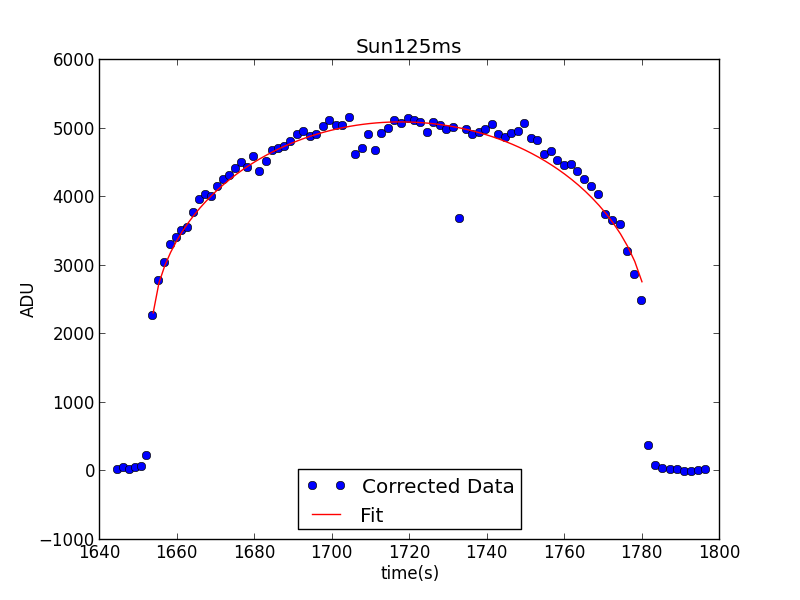
\includegraphics[scale=0.4]{11.png}
  \caption{This figure shows the intensity vs. time of sun with integration time of 125ms. The blue dots show the averaged spectra across the sun and the red curve shows the fit to the data. There is one dot really off from the other points which has been removed from the data for correlations that come later in the sections.}
  \label{fig:minipage1}
\end{minipage}
\quad
\begin{minipage}[b]{0.4\linewidth}
  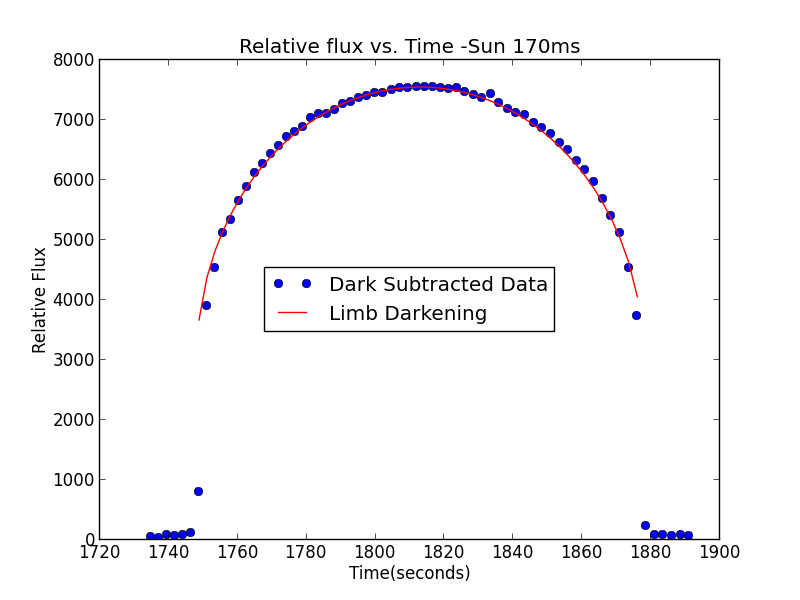
\includegraphics[scale=0.4]{sun170ms.png}
  \caption{This figure shows the intensity vs. time of sun with integration time of 170ms. Similar to the left picture, the blue dots show the averaged spectra and the red curve is the fit to these data points. We did not remove any of the points from the data.}
\label{fig:minipage2}
\end{minipage}
\end{figure}


\subsection{Flattening and Smoothing}
We  wanted to make the solar spectrum to look flat rather than having a blackbody shape since it is easier to see the features such as the shift and also the absorption lines. In order to do so, I tried different methods which some worked and some did not. Here I will go over the methods. First of all, I tried fitting a blackbody curve to it with considering the surface temperature of the sun (5777 K), but since the spectrum is covering only a small range of the wavelength, the blackbody values did not change much and therefore division of the spectrum by the black body basically did nothing. The second method I used was using  smoothing Python code found online called savitzky\_golay.py . This code generated a function that had a similar overall shape of our data. We should note that we should use large window sizes so that by smoothing we do not loose spectral features. Then by dividing our data by this smoother function we can get rid of the slope in the spectrum and still preserve the spectral features. However, this generated huge amount of noise at the end of the spectrum since we did not have much information on the end parts of the spectrum so the noise(uncertainty) on the end points got big. Therefore, I used a third method using gaussian functions, and it worked better than the others in that it flattened the spectrum and reduced the amount of noise at the end parts. The code explanation can be found in Appendix.


\subsection{Velocity Resolution of Spectrometer}
Each spectrometer has a specific velocity resolution which corresponds to its wavelength and therefore, its pixel resolving power. We used Mercury peak in the wavelength range of 523nm-573nm (since t only has one peak in this wavelength range) in order to compute this velocity resolution. The method we used is that we fitted a gaussian function on the peak and calculated the Full Width half Maximum(FWHM) which is given by Eq. [...]:

\begin{equation}
FWHM=2\sqrt{n\ln 2}  \sigma
\end{equation}
where $\sigma$ is the standard deviation of the data. We found the $\sigma$ for the gaussian fit to be 2.816 $\pm$7.0532e-05 pixels which corresponds to FWHM of 3.315 $\pm$ 7.0532e-05pixels and by Eq. [...] this gives the velocity resolution of about 29.885 km/s, which is close to the 33 km/s value given in the lecture slides. The percentage difference is 9.44 \% which is good enough. Figure [...] shows the mercury 50ms peak and the gaussian fit on it.


% Gaussian fit image
\FloatBarrier
\begin{figure}[h!]
\centering
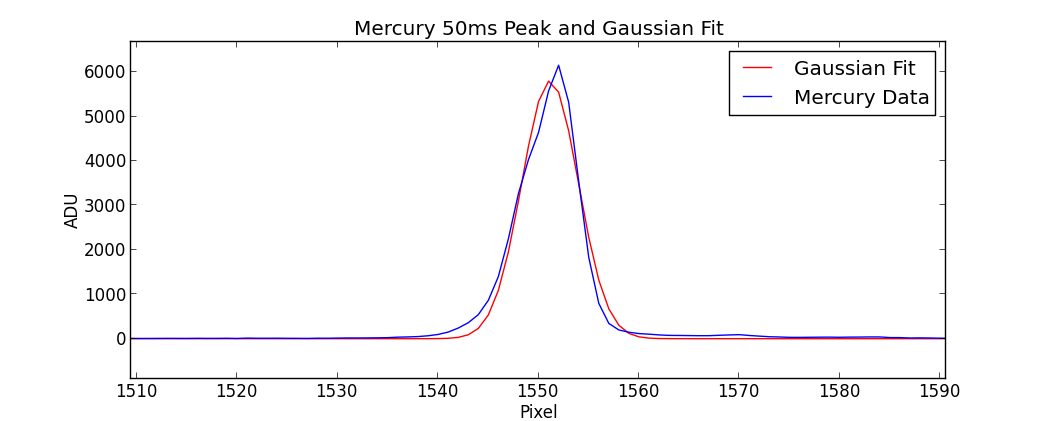
\includegraphics[scale=0.48]{velocity_resolution.png}
\caption{This figure shows the mercury 50ms peak in blue and the gaussian fit on to of it in red. We then computed the $\sigma$ of the gaussian function and used it to calculate FWHM of it in order to find the velocity resolution of the spectrometer using Doppler Shift Equation.}
\end{figure}
\FloatBarrier


\section{Determining Doppler Shift}
\label{sec:determiningdopplershift}
As we were collecting the solar data, the sun was rotating. We need to account this rotation since it affects the wavelength of the light that we observe. As the sun rotates, one edge is turning toward us, making the light to appear blue-shifted(light has shorter wavelength) and the other edge is turning away from us, making it to appear red-shifted(light has longer wavelength). This is known as Doppler Shift and it is given by equation [...]:

\begin{equation}
\frac{\Delta \lambda}{\lambda}=\frac{\Delta v}{c}=\frac{2 v_{rad}}{c}
\end{equation}

\begin{equation}
v_{rad}=\frac{c\Delta \lambda}{2\lambda}
\end{equation}


Where $\Delta v$ is the change in velocity, $\Delta \lambda$ is the change in wavelength given some reference wavelength, $\lambda$ and $c$ is the speed of light in vacuum. The spectrometer we used has a 
velocity resolution of 33 km/s. Figure [...] shows the spectrums of the two edges of the sun. As it can be seen in the image, even the two furthest spectrums are very close to each other.


\FloatBarrier
\begin{figure}[h!]
\centering
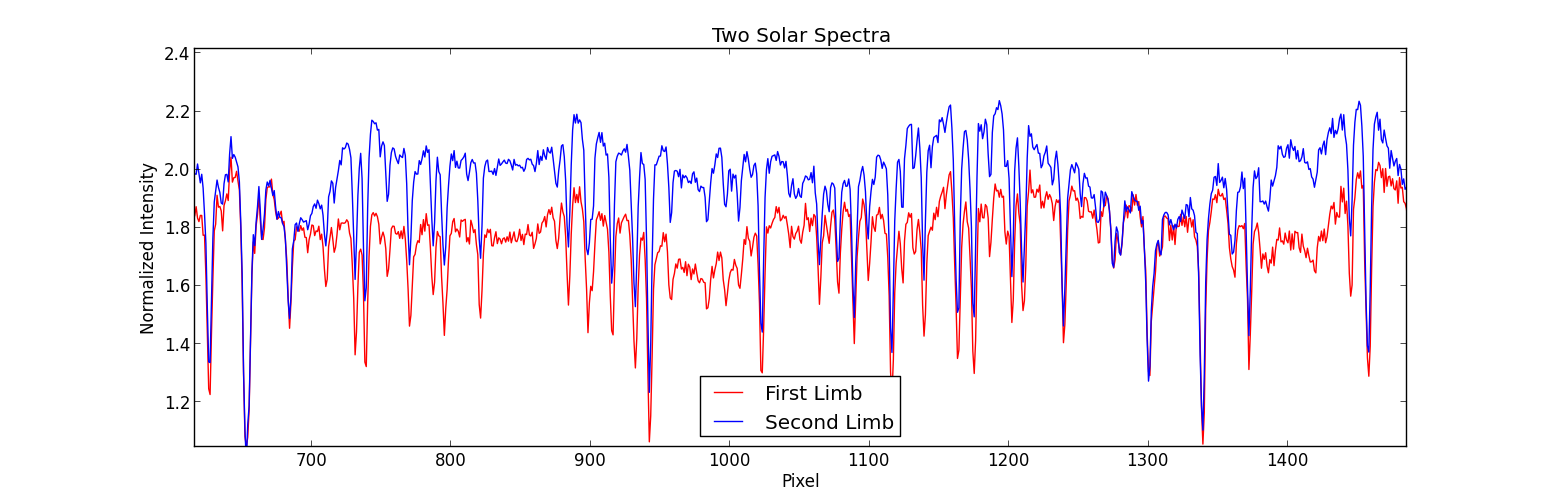
\includegraphics[scale=0.4]{limbs.png}
\caption{$Top:$Two spectra of the two edges of the sun over-plotted. As it can be seen, the two spectra are very close to each other. $Bottom:$ The two spectra are zoomed so the features are better shown.}
\end{figure}
\FloatBarrier


\subsection{Cross-Correlation}
Cross-correlation is a method used in this lab in order to show how similar the different spectra are with respect to a reference spectrum of the sun. Covariance is a statistical parameter that shows how correlated two variable are. Covariance can be computed by Eq. [...]:

\begin{equation}
s_{j}^2=\frac{1}{N-1}\Sigma (x_{i}-\bar x)(y_{i}-\bar y)
\end{equation}
Where N is the size of the data set, $\bar x$ and $\bar y$ are the mean values of the two data sets. In theory, the maximum value of the covariance shows where the two data sets are most similar. In order to find the shift in the pixel values of the two data sets, we considered an array from -10 to 10 and iterated it by 1 pixel each time, and computed the covariance. Then we plotted covariance vs. the array we formed. Then we should find the centroid of the cross-correlation in order to find the pixel shift. This can be computed by Eq. [...]:
\begin{equation}
<j>=\frac{\Sigma_{j}jX_{j}}{\Sigma_{j}X_{j}}
\end{equation}

% Fourier Transorm
\subsection{Fourier Transform}
A Fourier Series is where any function expressed as the sum of sines and cosines.


\subsection{Window Function}
In applying cross-correlation we shift the spectra relative to one another. In doing so, we beginning and the tail of the spectra would not match and line up with other spectra since our data set is finite. Since our data is discrete (we cannot integrate from [-inf] to [inf], causes the energy from the true frequency to "leak" into adjacent frequencies. Leakage is one of the most common digital signal processing errors and it cannot be eliminated completely, it can only be minimized. Therefore, we could use the window functioning method that weights the beginning and end values of the data set to zero and it also minimizes edge effects and leakage of frequencies and amplitude of the signal. In this lab we used the Hanning window function which is given by Eq. [...] below, where M is the number of points we want the window function to return:

\begin{equation}
w(n)=0.5(1-\cos (\frac{2\pi n}{M-1}))  %  0\<n\<(M-1)
\end{equation}
It is used for smoothing and it is also known as apodization which means that it "removes the foot", i.e.smoothing discontinuities at the beginning and end of the sampled signal) or tapering function.



\section{Discussion}
\label{discussion}
Using the methods discussed in section 4, we computed the pixel shift from the two end spectra using the one that starts earlier as the reference spectrum. Then we used the wavelength solution we found for the spectrometer to convert this pixel shift into wavelength shift so that we could use Doppler Shift equation given by Eq. [..] to compute the radial velocity of the Sun. The pixel shift found is -0.511 which corresponds to approximately -0.008 nm shift in the wavelength. The radial velocity then would be -2.30 km/s .

Figures [..] and [...] show the spectrum of the beginning of the sun and the plot of the window function applied to the same data, respectively.

% window functions
\begin{figure}[ht]
\centering
\begin{minipage}[b]{0.5\linewidth}
  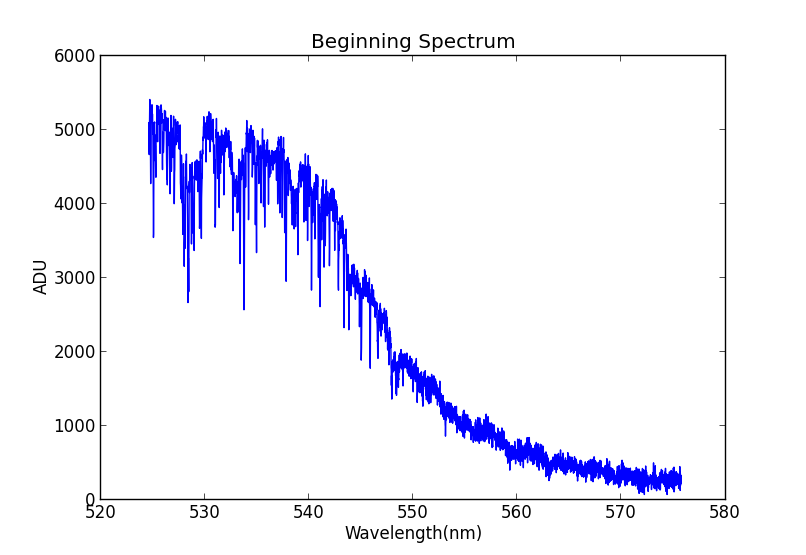
\includegraphics[scale=0.4]{file1.png}
  \caption{This figure shows the intensity vs. wavelength of beginning of the solar spectrum. This is dark subtracted and divided by flat.}
  \label{fig:minipage1}
\end{minipage}
\quad
\begin{minipage}[b]{0.4\linewidth}
  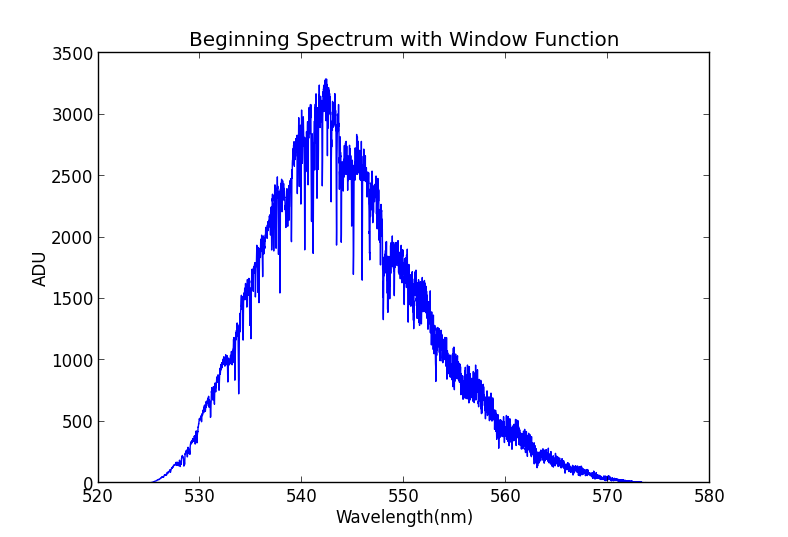
\includegraphics[scale=0.4]{windofile1_windowed.png}
  \caption{This figure shows the beginning spectrum of the sun which Hanning window function is applied on.}
\label{fig:minipage2}
\end{minipage}
\end{figure}

After applying the window function to the spectra, I recalculated the pixel shift and it was 0.508, so there is a small change in the pixel shift when window function was applied.

In order to find AU, we also need to find the angular size and radius of the Sun that are given by Eq. [..] and Eq. [...], respectively.
%angular size equation
\begin{equation}
\frac{\Delta t}{24 h}=\frac{\theta}{360^{o}}
\end{equation}


% v real
\begin{equation}
v_{real}=\frac{v_{rad}}{\cos(\eta) \cos(\xi)}
\end{equation}

% R sun equation
\begin{equation}
R_{sun}=\frac{v_{real} T}{2 \pi}
\end{equation}

Using simple geometry, we can finally find the distance D, which is the distance between the Sun and the Earth. Fig. [...] shows the sketch of the geometry and the math is shown in Eq. [..].

\begin{equation}
D=\frac{R_{sun}}{\tan (\theta/2)}
\end{equation}

Here, $\Delta t$ is the time between the two limbs of the sun which is twice the $\Delta t$ we used to plot the limb darkening, therefore, $\Delta t$ is 126.138 s, which is equal to 2.1023 minutes. Using Eq. [...] $\theta$ has a value of 0.5334 degrees. The true angular size of the sun is approximately 0.5331 degrees as given on JPL HORIZONS [... reference] for the day of our observation, so the percentage difference with my value and the value on JPL is  0.06 \%, which is very accurate.

% simple geometry sketch
\FloatBarrier
\begin{figure}[h!]
\centering
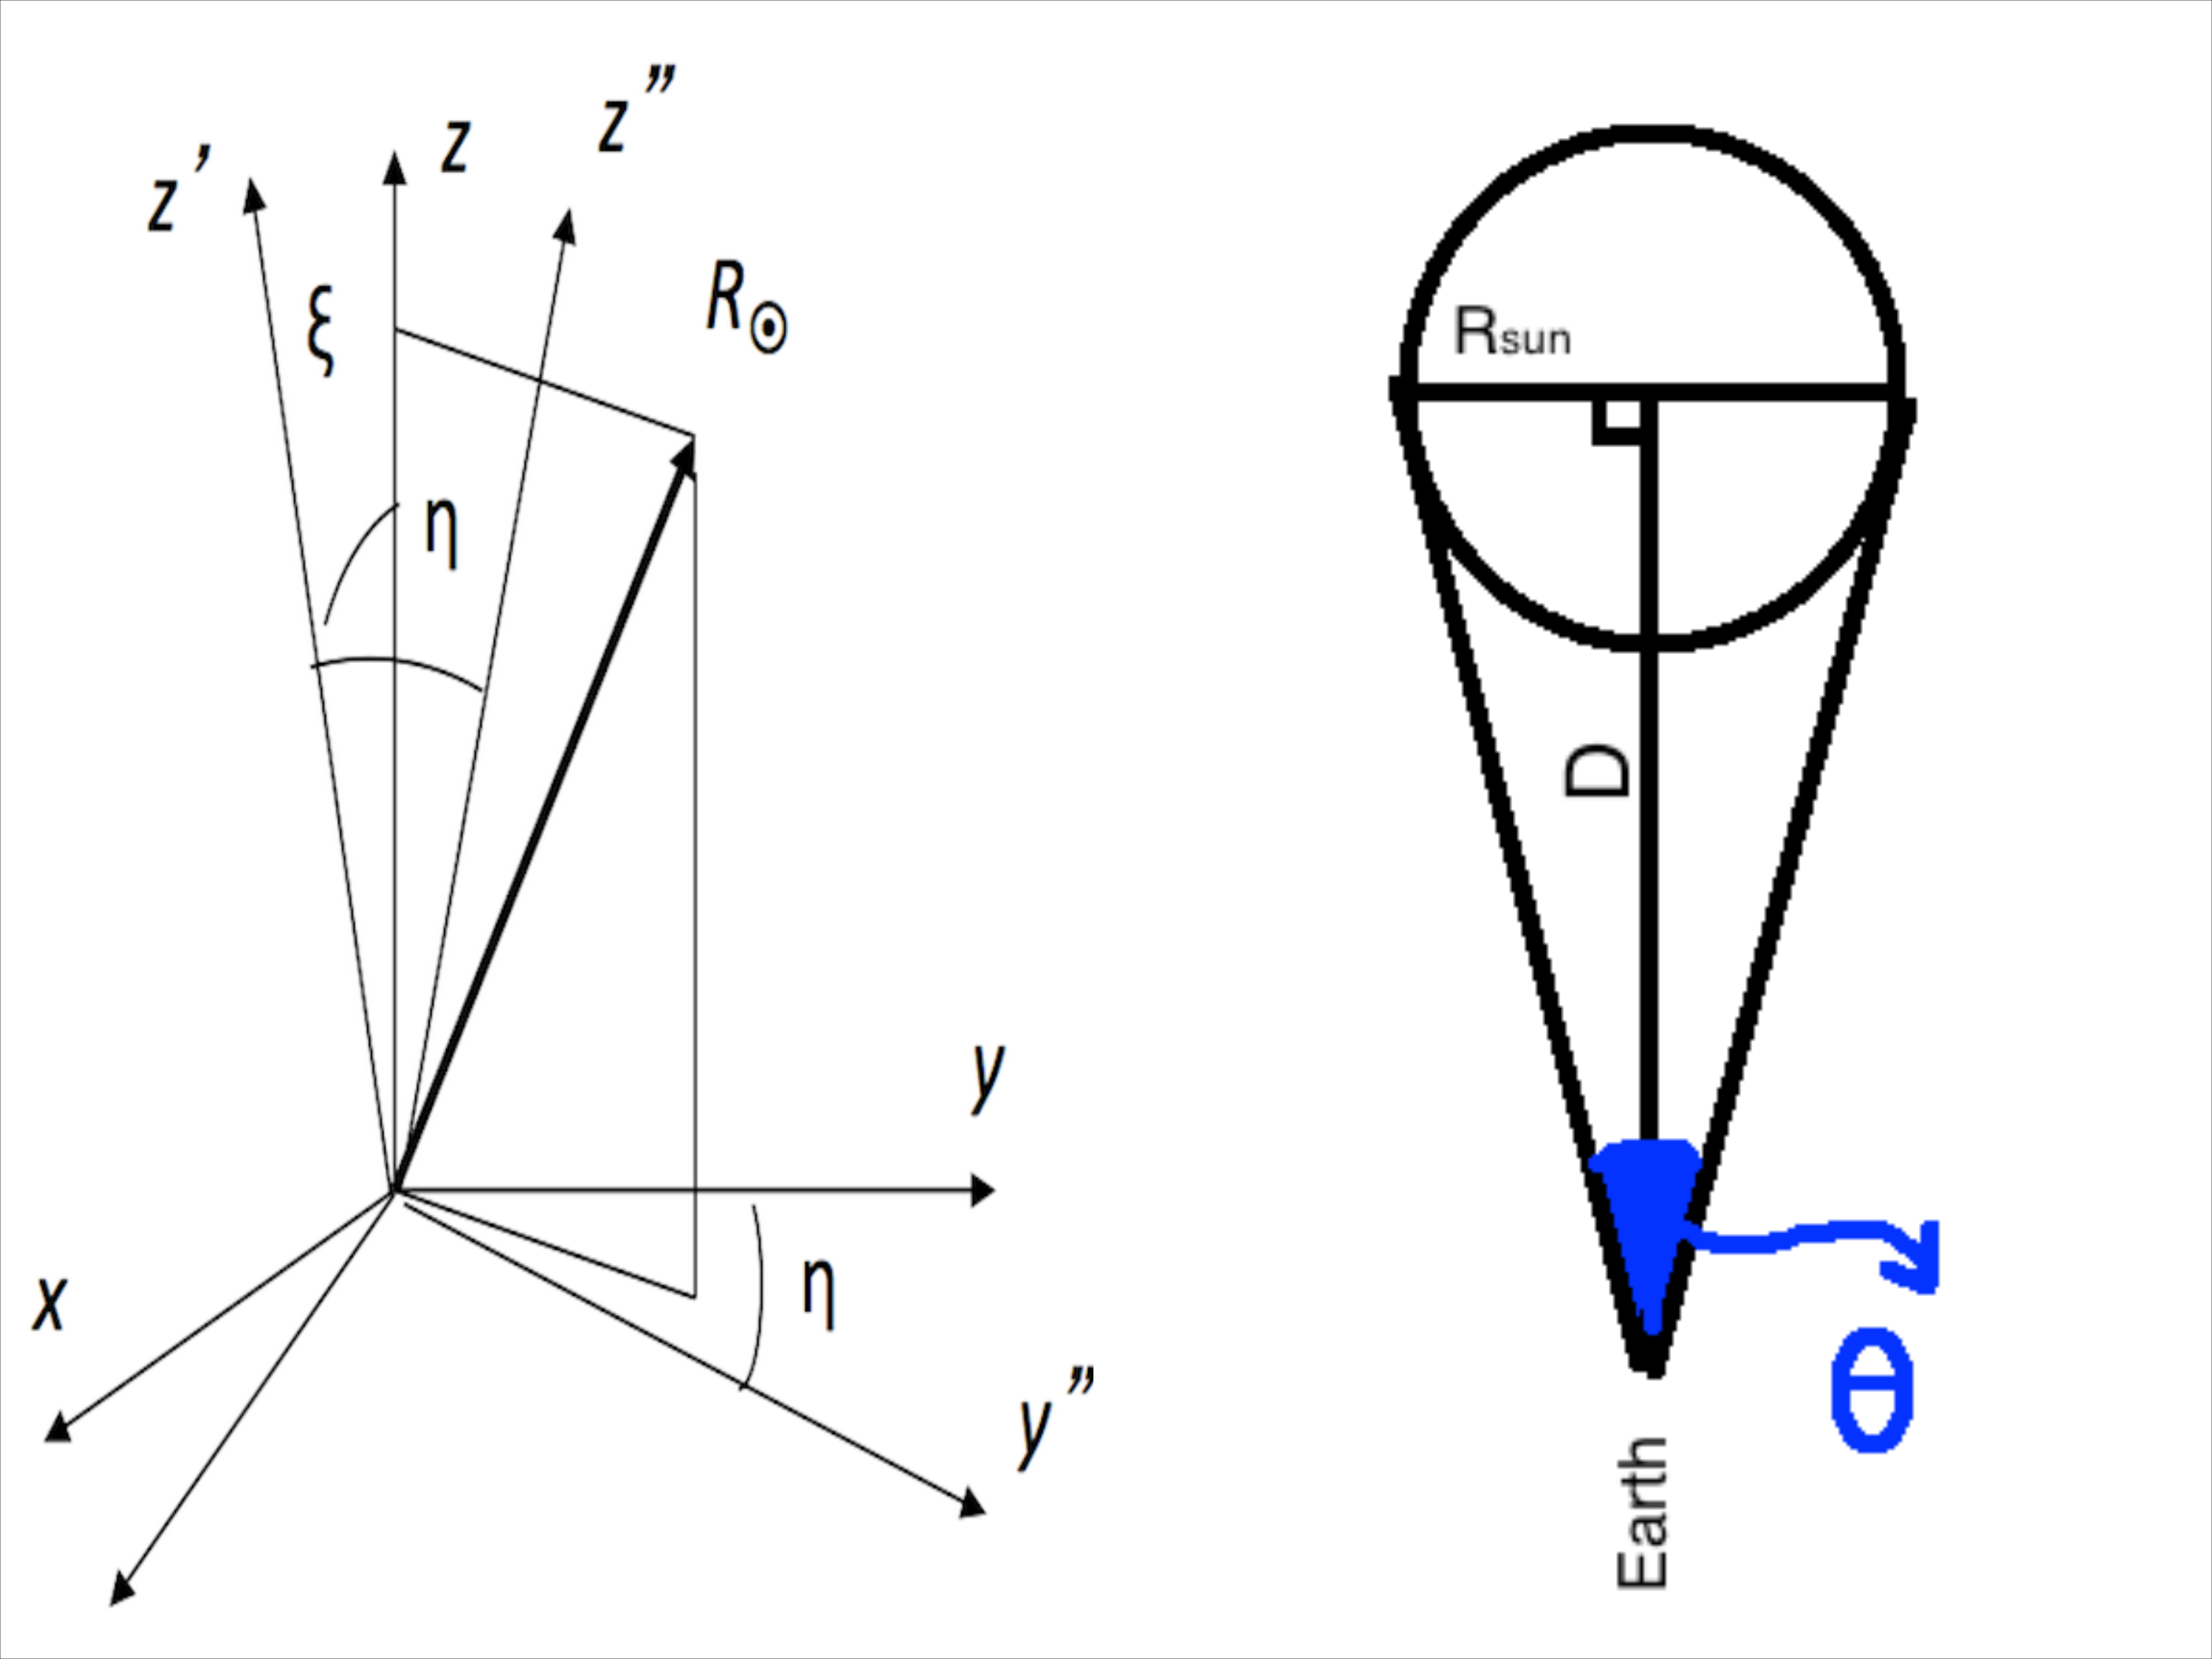
\includegraphics[scale=0.1]{transformation.png}
\caption{$Left:$Shows coordinate transformation for solar axis since it is not perpendicular to the ecliptic, meaning that the center of the sun as viewed from Earth is not b=0. Therefor, we should rotate it about y-axis by the angle $\xi$ and about x-axis by the angle $\eta$ .$Right:$This is a sketch of the simple geometry for calculating the AU using the computed values of angular size of the sun and its radius.}
\end{figure}
\FloatBarrier


\subsection{Error Analysis}




\section{Conclusion}
\label{sec:conclusion}


\section{References}
\label{sec:references}
1-http://www.aseq-instruments.com/HR1.html
\\*2-http://en.wikipedia.org/wiki/Angular\_diameter
\\*3-The lecture slides


\section{Appendix}
\label{sec:appendix}

We first discuss how we found the peaks of the spectrum of neon and mercury using centroid method. Below is the code I used to find the centroids. It goes through all of the pixels and checks the intensity value of each pixel with its neighbour pixel intensity value. If it is higher than both its left and right pixels it points as a peak.
\begin{verbatim}
for i in range(0,3652,1):
    if values[i+1]>values[i]:
        i+=1
        if values[i+1]<values[i]:
            if values[i]>70:
                Pixellist.append(i)
                centroidintensity = 0.5*(values[i]+values[i+1])
                centroidintensitylist.append(centroidintensity)
\end{verbatim}
Here is how fitting wavlength vs. pixel values work using linear sqaures.
\begin{verbatim}
ma =np.array([[np.sum(Pixels**2),np.sum(Pixels)],[np.sum(Pixels),len(Pixels)]])
mc =np.array([[np.sum(Pixels*Wavelengths)],[np.sum(Wavelengths)]])  #matrices
mai = np.linalg.inv(ma)
md = np.dot(mai,mc)
\end{verbatim}

Next, we will discuss how the times of the solar observations were extracted from the file names.
\begin{verbatim}
times=[]
for k in range(0,66,1):
    names=np.loadtxt('sun170ms-filenames.txt',dtype='str')
    minutes=names[k][17:19]      # taking minute parts of the file name
    minutes=float(minutes)*60    # converting str to int and converting to seconds
    seconds=names[k][19:21]     # taking second parts of the file name
    seconds=float(seconds)        # converting str to int
    miliseconds=names[k][21:24] # taking mili second parts of the file name
    miliseconds=float(miliseconds)/1000 #converting str to int and to seconds
    time=minutes+seconds+miliseconds
    times.append(time)
t_center=times[5]+(times[59]-times[5])
Delta_t=(times[59]-times[5])/2
I_o=7550  #central intensity
I=I_o*((2./5)+((3./5)*(np.sqrt(1-(((times-t_center)**2)/(Delta_t**2))))))    
\end{verbatim}





\end{document}